\section{Appendix}

\subsection{Refining English G2P}
\label{sec:appendix-engg2p}
We observed confusion in plosive voice-onset times on unseen languages in preliminary experiments, which is likely from English G2P data. For instance, broad phonemic transcription in English typically uses /b/ to transcribe the /b/ in /bat/, but its voice onset timing is actually voiceless in Mainstream American English and is closer to [p]. To mitigate this, we apply rule-based refinements to English G2P transcriptions, adjusting plosive voicing and aspiration, lateral velarization, and vowel nasalization.

The rules are listed below: 
1) word-initial voiceless plosives (\textipa{/p/, /t/, /k/}) are aspirated,
2) word-initial voiced plosives (\textipa{/b/, /d/, /g/}) are voiceless, 
3) lateral \textipa{/l/} is velarized at the end of syllables, and 
4) vowel nasalization before nasal consonants.


\subsection{Baseline Implementation}
\label{sec:appendix-baseline}
We provide the baselines' training data source, number of languages covered in the data, and links to model checkpoints or repository in \autoref{tab:training-data-summary}.

\begin{table*}[t]
\centering
\small
\resizebox{\textwidth}{!}{
%\begin{tabular}{@{}l p{4cm} c p{5cm}}
\begin{tabular}{ll c l}
\toprule
\textbf{Model} & \textbf{Training Data Sources} & \textbf{Language Coverage} & \textbf{Model checkpoint / GitHub} \\
\midrule
\textbf{PR baselines}\\
\addlinespace[0.10cm]

\textbf{Allosaurus} & VoxForge,  Japanese CSJ, Hkust & \multirow{2}{*}{12} & \href{https://github.com/xinjli/allosaurus}{xinjli/allosaurus}  \\
\cite{li2020universal,li2021hierarchical} & Tedlium, Switchboard etc & & \\
\addlinespace[0.15cm]

\textbf{Allophant} &\multirow{2}{*}{Common Voice 10.0} & \multirow{2}{*}{34} & \href{https://github.com/kgnlp/allophant}{kgnlp/allophant}  \\
\cite{glocker23_interspeech} & & &  \\
\addlinespace[0.15cm]

\textbf{Wav2Vec2Phoneme} & MLS, Common Voice, & \multirow{2}{*}{40+} &\multirow{2}{*}{{\href{https://huggingface.co/facebook/wav2vec2-xlsr-53-espeak-cv-ft}{facebook/wav2vec2-xlsr-53-espeak-cv-ft}}} \\
\cite{xu22b_interspeech} & Babel &  \\
\addlinespace[0.15cm]

\textbf{MultIPA} & \multirow{2}{*}{Common Voice 11.0} & \multirow{2}{*}{7} & \multirow{2}{*}{{\href{https://huggingface.co/ctaguchi/wav2vec2-large-xlsr-japlmthufielta-ipa1000-ns}{ctaguchi/wav2vec2-large-xlsr-japlmthufielta-ipa1000-ns}}} \\
\cite{taguchi23_interspeech} &\\
\addlinespace[0.15cm]

\textbf{ZIPA} & IPAPack++ & \multirow{2}{*}{88} & \href{https://github.com/lingjzhu/zipa}{lingjzhu/zipa} \\
\cite{zhu-etal-2025-zipa} & MMS ulab v2.,  VoxLingua-107 (Pseudo-label) & & \href{https://huggingface.co/anyspeech/zipa-large-crctc-ns-800k}{anyspeech/zipa-large-crctc-ns-800k} \\
\addlinespace[0.10cm]

\midrule
\textbf{ASR baselines}\\
\addlinespace[0.10cm]

\textbf{OWSM-CTC v4} & \multirow{2}{*}{OWSM v3.2, YODAS} & \multirow{2}{*}{100+} &\multirow{2}{*}{{\href{https://huggingface.co/espnet/owsm_ctc_v4_1B}{espnet/owsm\_ctc\_v4\_1B}}}\\
\cite{peng25c_interspeech} \\
\addlinespace[0.15cm]

\textbf{OWLS} & \multirow{2}{*}{OWSM v3.2, YODAS} & \multirow{2}{*}{150} &\multirow{2}{*}{{\href{https://huggingface.co/collections/espnet/owls-scaling-laws-for-speech-recognition-and-translation-67ab7f991c194065f057ce8d}{espnet/owls-scaling-laws-for-speech-recognition-and-translation}}}\\
\cite{chen2025owls}\\

\bottomrule
\end{tabular}
}
\caption{Overview of the baselines for our work.}
\label{tab:training-data-summary}
\end{table*}


\subsection{FLEURS language selection for ASR}
\label{sec:appendix-asr-splits}
We first filter out languages with more than 8 hours of training data in IPAPack++ \cite{zhu-etal-2025-zipa}, keeping only those that are also present in FLEURS.
Then, following the training data amounts reported in \citet{chen2025owls}, we further identify the 50 lowest-resource languages to exclude any that may have other substantial sources not included in IPAPack++.
This process leaves us with nine languages. We finally exclude \texttt{ell}, as it is comparatively higher-resource and because there are already three other Balto-Slavic languages.
Note that other models use strictly more data than ours---not only in terms of dataset count but also because IPAPack++ applies additional data-quality filtering. \autoref{tab:asr-data-stats} lists the amount of ASR training data for baselines.

\begin{table}[h]
\vspace{-2mm}
\centering
\small
\setlength{\tabcolsep}{4pt} % Adjust column spacing
\renewcommand{\arraystretch}{1.4}
\resizebox{\columnwidth}{!}{
\begin{tabular}{l cc c cc ccc}
\toprule
% use numbers reported in OWSM v4
& \multicolumn{2}{c}{Afroasiatic} & Turkic & \multicolumn{2}{c}{Indo-Iranian} & \multicolumn{3}{c}{Balto-Slavic}\\
Model & \texttt{afr} & \texttt{orm} & \texttt{aze}  & \texttt{pan} & \texttt{tgk}  & \texttt{mkd} & \texttt{bos} & \texttt{slv}\\
\midrule
POWSM & 2.71 & 5.11 & 6.89 & 4.96 & 6.52 & 5.14 & 7.57 & 7.19 \\
OWSM-CTC v4 & \multirow{2}{*}{5.54} & \multirow{2}{*}{6.50} & \multirow{2}{*}{10.69} & \multirow{2}{*}{8.30} & \multirow{2}{*}{8.03} & \multirow{2}{*}{8.4} & \multirow{2}{*}{9.96} & \multirow{2}{*}{26.00} \\
OWLS & \\
\bottomrule
  \end{tabular}
}
 \caption{Amount of ASR training data for languages included in ASR comparison (in hours), according to \citet{zhu-etal-2025-zipa} and \citet{chen2025owls}.}
 \label{tab:asr-data-stats}
% \vspace{-2mm}
\end{table}


\begin{figure*}
    \centering
    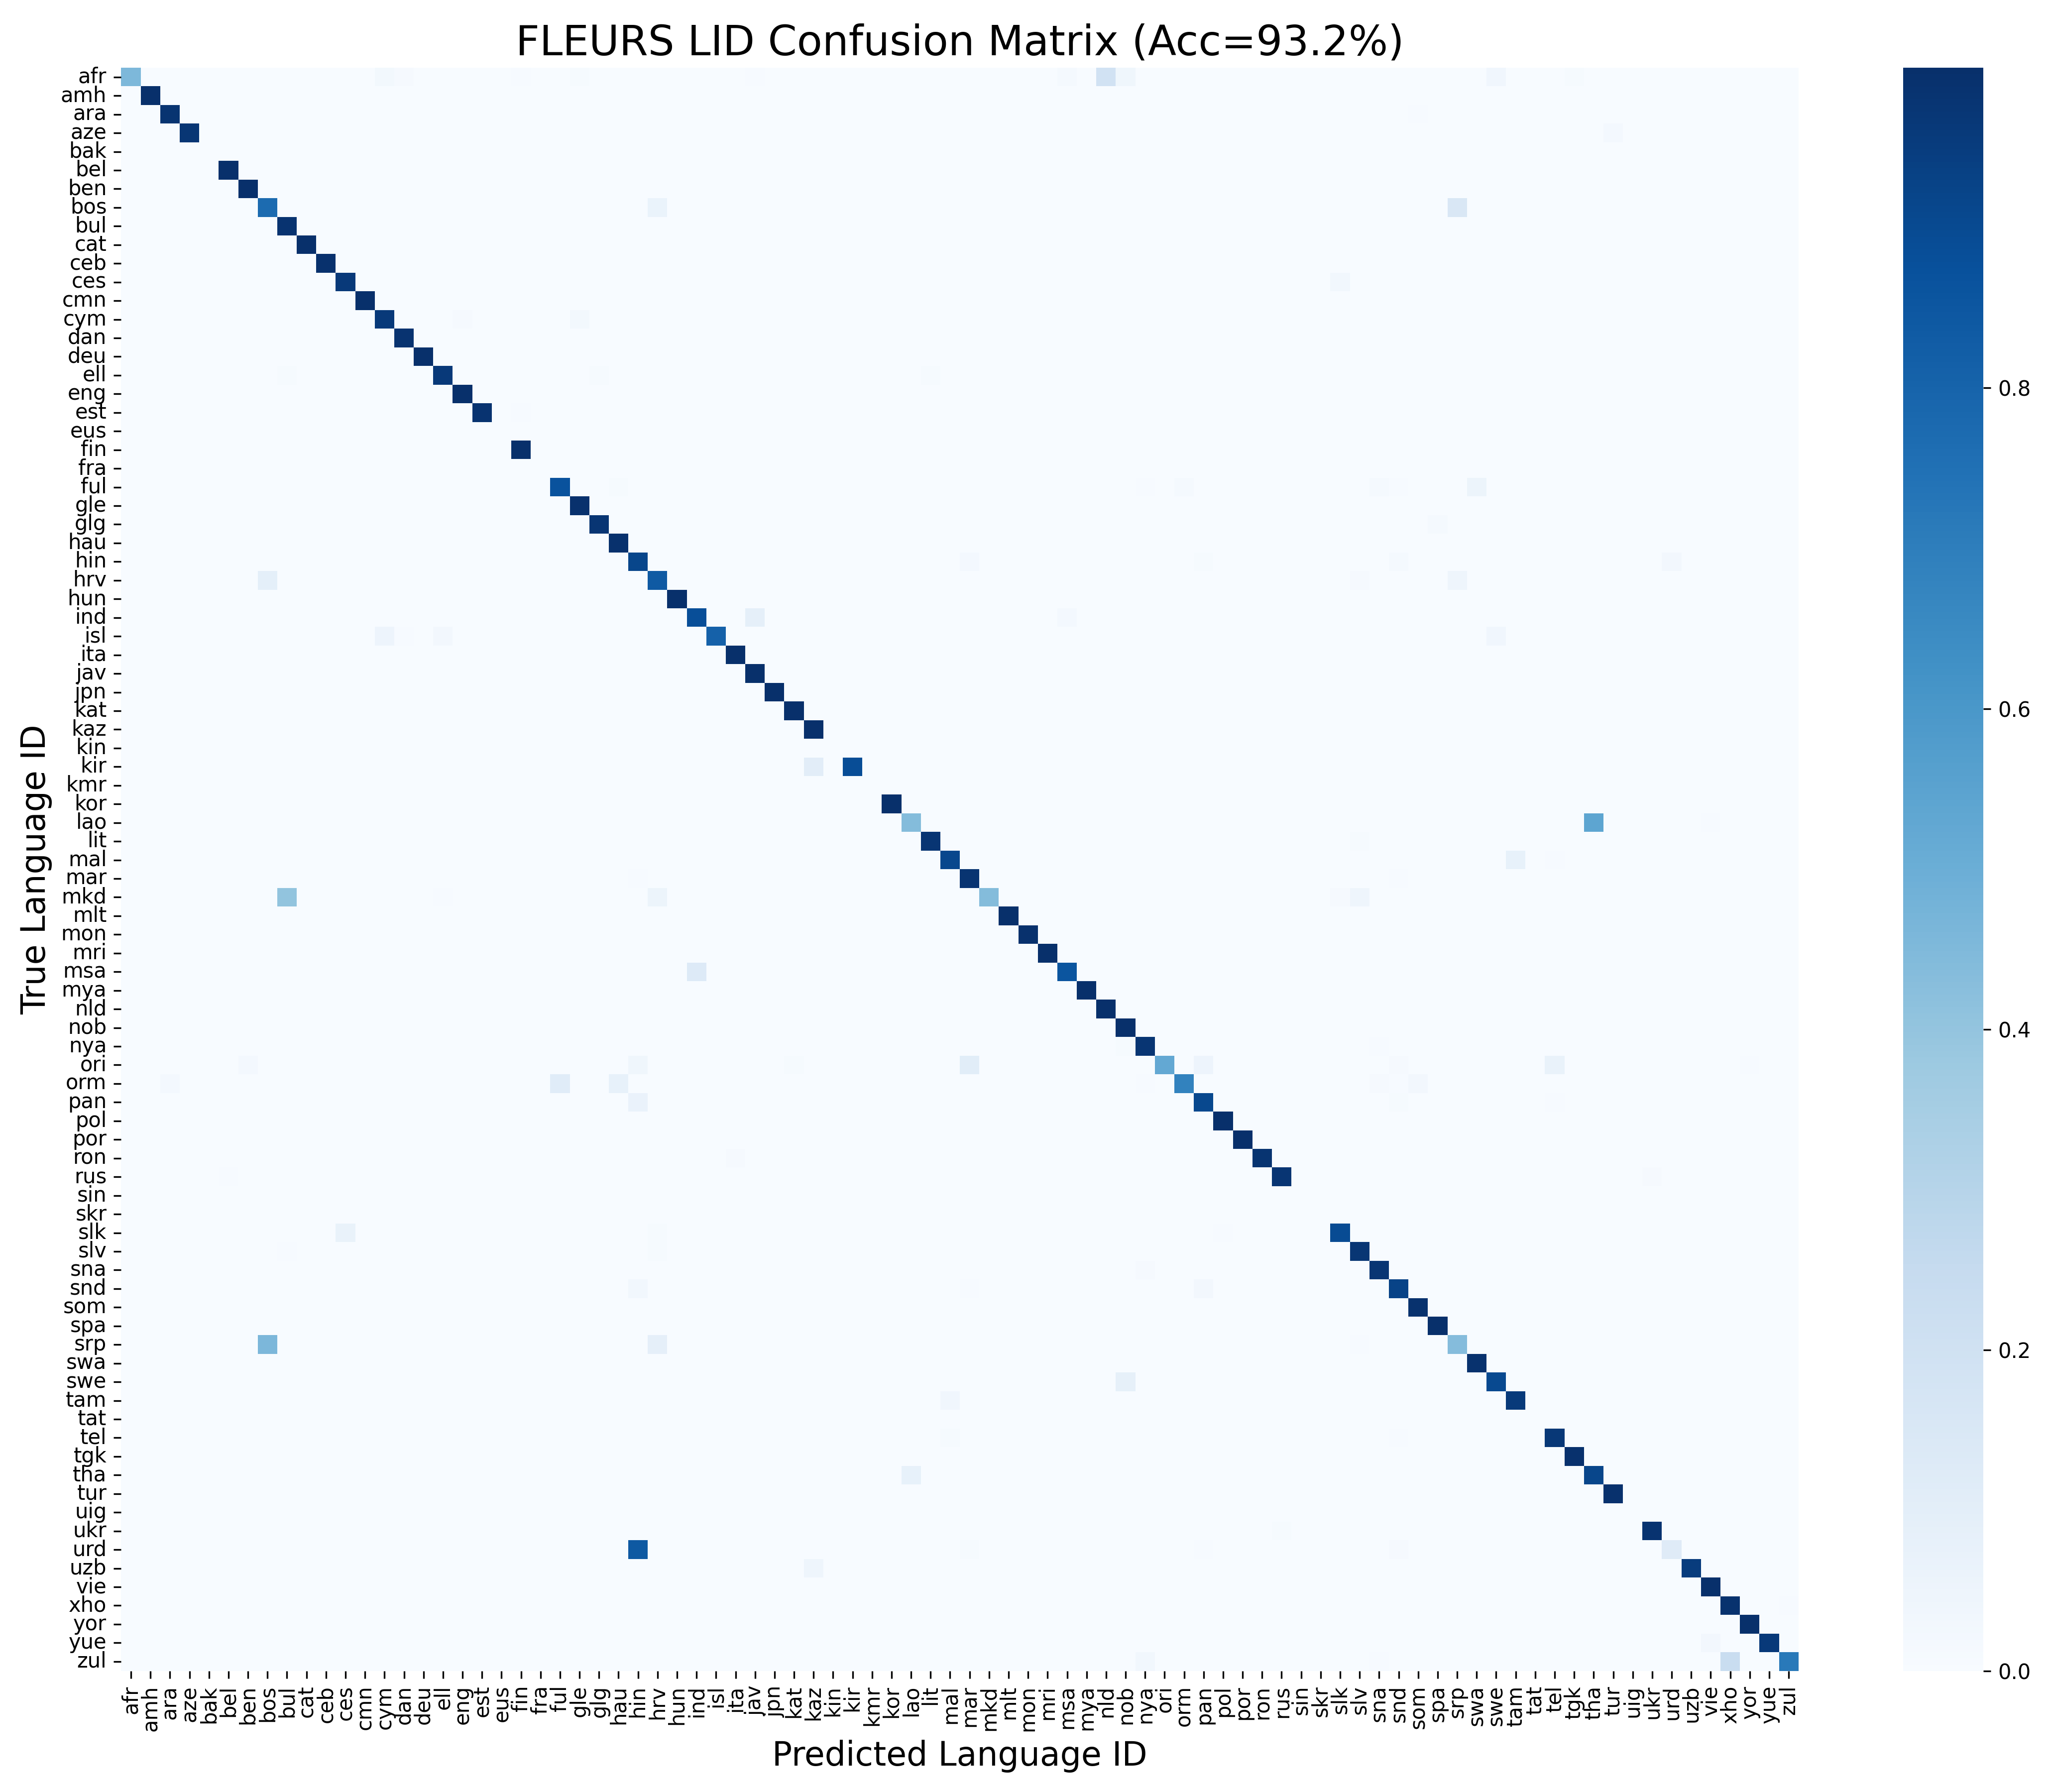
\includegraphics[width=0.8\textwidth]{figures/fleurs_lid.png}
    \caption{Confusion matrix of LID on FLEURS.}
    \label{fig:lang-token-seen}
\end{figure*}

\subsection{ASR Performance on In-Domain Data}
\label{sec:appendix-asr-perf}
We run greedy decoding (\texttt{ctc=0.0, beam=1}) on the test sets of in-domain data. 
\autoref{tab:asr-hrl} shows that ASR performance is reasonably competitive with previous models \cite{radford2023robust, peng25c_interspeech} of similar size and architecture despite being trained on much fewer data. 
The performance gap is smaller for languages that constitute a larger portion of the training data, and larger for mid-frequency languages.
Errors often involve substitutions of phonetically similar words or phrases (e.g., \textit{``mostly rapscallions as fur''} to \textit{``mostly wrapped skaggins as fer''}).

\begin{table}[h]
\centering
\small
\setlength{\tabcolsep}{4pt} % Adjust column spacing
\renewcommand{\arraystretch}{1.2}
\resizebox{\columnwidth}{!}{
\begin{tabular}{l ccc ccc ccc cc}
\toprule
& \texttt{eng} & \texttt{deu} & \texttt{nld} & \texttt{fra} & \texttt{ita} & \texttt{spa} & \texttt{por} & \texttt{pol} & \texttt{tam} & \texttt{kaz} & \texttt{cmn} \\
\midrule 
\POWSM & --- & 11.5 & 20.2 & 13.8 & 23.6 & \wpad9.4 & 25.7 & 31.0 & 40.4 & 23.4 & 21.9 \\
\POWSM-fix & 12.2 & 12.7 & 19.5 & 13.9 & 22.2 & 11.3 & 25.5 & 28.5 & 32.6 & 14.8 & 21.7 \\
Whisper & \wpad8.3 & 11.5 & 18.2 & 13.6 & 21.3 & \wpad9.1 & 13.8 & \textbf{12.5} & --- & --- & 26.6 \\
OWSM & \textbf{\wpad4.7} & 10.3 & 15.7 & 14.1 & 21.8 & \wpad7.1 & 11.5 & 16.0 & --- & --- & \textbf{14.9}\\
\midrule
OWSM-CTC & \wpad5.1 & \textbf{\wpad9.5} & \textbf{15.1} & \textbf{\wpad7.8} & \textbf{15.5} & \textbf{\wpad5.8} & \textbf{10.3} & 15.1 & --- & --- & 18.7\\
\bottomrule
  \end{tabular}
 }
\caption{WER ($\downarrow$) on test sets; \texttt{cmn} reports CER ($\downarrow$). \textit{POWSM-fix} is discussed in \autoref{sec:appendix-textissue}. 
\textit{Whisper} (Whisper-small) and \textit{OWSM} (OWSM v4 small) are models of similar size and architecture, trained with 10 times more data. \texttt{tam} and \texttt{kaz} are omitted due to normalization issues; Whisper outputs numerals for \texttt{cmn}, inflating its CER. }
\label{tab:asr-hrl}
\end{table}


\subsection{Multi-tasking at Different Scales}
\label{sec:appendix-multitask}
Multi-tasking may improve performance by tying acoustic signals to well-defined symbolic representations, yet it may distract the model if the relationships are not learned effectively. 
We train \POWSM with different data and model scales to examine how multitask learning interacts with the setup, and use \texttt{beam=1} during decoding to speed up inference.

\autoref{tab:multitask-small} shows that there is no clear trend regarding whether multitasking benefits PR performance. PR performance  degrades when the model has excessive capacity relative to the available data (too little data), or when it is limited by size (too much data).

Further evidence is needed before concluding that phoneme recognition benefits less from scaling, as we currently lack sufficient data and large model capacity to test this thoroughly. Nevertheless, the model demonstrates the ability to multitask, which represents a promising direction for future work. 

% \autoref{tab:multitask-small} shows that in a low-resource setting, multi-tasking consistently improves performance as more tasks are added. However, the gains saturate with larger data and models, echoing prior findings \citep{chen2025owls} that less language-dependent tasks such as phone recognition benefit less from scaling.
% Our results contradict ``How Phonotactics Affect Multilingual and Zero-Shot ASR Performance''
% ``We show that the gain from modeling crosslingual phonotactics is limited, and imposing a too strong model can hurt the zero-shot transfer. Furthermore, we find that a multilingual LM hurts a multilingual ASR system’s performance, and retaining only the target language’s phonotactic data in LM training is preferable.''

\begin{table}[h]
\centering
\small
\setlength{\tabcolsep}{4pt} % Adjust column spacing
\renewcommand{\arraystretch}{1.2}
\resizebox{\columnwidth}{!}{
\begin{tabular}{c c c c c c}
\toprule
Data ( khr) & Tasks & Params. & VoxAngeles & Tusom2021 & L2-Arctic \\
\midrule 
0.25 & 1 & 100M & 27.22 & 32.59 & 13.50\\
0.25 & 4 & 100M & 26.30 & 30.32 & 13.40\\
0.25 & 1 & 300M & 20.63 & 25.83 & 12.88\\
%0.25 & 2 & 300M & 20.10 & 27.53 & \\
0.25 & 4 & 300M & 23.81 & 25.91 & 14.14\\
\midrule
17 & 1 & 100M & 17.88 & 26.68 & 11.76\\
17 & 2 & 100M & 24.69 & 49.28 & 11.35\\
17 & 4 & 100M & 30.07 & 61.89 & 12.37\\
17 & 1 & 300M & 17.08 & 25.20 & 10.50\\
17 & 2 & 300M & 17.17 & 23.70 & 10.47\\
17 & 4 & 300M & 17.58 & 33.52 & 10.54\\
\bottomrule
  \end{tabular}
 }
\caption{Comparison of PFER ($\downarrow$) on different seting of tasks and data. 1 task refers to PR, 2 tasks refer to PR+ASR, and 4 tasks include PR, ASR, P2G, and G2P.}
\label{tab:multitask-small}
\vspace{-2mm}
\end{table}


\subsection{DoReCo \citep{paschen2020doreco}}
\label{sec:appendix-doreco}

DoReCo consists of the following constituent datasets: \citep{
doreco-anal1239,
doreco-apah1238,
doreco-arap1274,
doreco-bain1259,
doreco-beja1238,
doreco-bora1263,
doreco-cabe1245,
doreco-cash1254,
doreco-dolg1241,
doreco-even1259,
doreco-goem1240,
doreco-goro1270,
doreco-hoch1243,
doreco-jeha1242,
doreco-jeju1234,
doreco-kaka1265,
doreco-kama1351,
doreco-kark1256,
doreco-komn1238,
doreco-ligh1234,
doreco-lowe1385,
doreco-movi1243,
doreco-ngal1292,
doreco-nisv1234,
doreco-nngg1234,
doreco-nort2641,
doreco-nort2875,
doreco-orko1234,
doreco-pnar1238,
doreco-port1286,
doreco-resi1247,
doreco-ruul1235,
doreco-sadu1234,
doreco-sanz1248,
doreco-savo1255,
doreco-sout2856,
doreco-sout3282,
doreco-stan1290,
doreco-sumi1235,
doreco-svan1243,
doreco-taba1259,
doreco-teop1238,
doreco-texi1237,
doreco-trin1278,
doreco-tsim1256,
doreco-urum1249,
doreco-vera1241,
doreco-warl1254,
doreco-yong1270,
doreco-yuca1254,
doreco-yura1255}.


\subsection{Fixing ASR Text Normalization}
\label{sec:appendix-textissue}
After submission, we discovered a text normalization issue specific to Librispeech that degraded its ASR performance. 
Continuing training with the corrected data for 20 GPUs hours on H100s mostly solved the problem (WER=14.2). 

Additionally, we trained a model from scratch with updated data, denoted as \textit{POWSM-fix}, where ASR transcripts are lowercased and punctuation is removed except for apostrophes and hyphens.
As shown in \autoref{tab:asr-hrl}, ASR performance is similar or improved, while \autoref{tab:powsm-fix} shows comparable PR performance on out-of-domain data when decoding with \texttt{ctc=0.3, beam=1}, enabling faster inference.
Both checkpoints are publicly available on HuggingFace for reproducibility.

\begin{table}[h]
\centering
\small
\setlength{\tabcolsep}{2pt} % Adjust column spacing
\renewcommand{\arraystretch}{1.2}
\resizebox{\columnwidth}{!}{
\begin{tabular}{l ccc ccccc}
\toprule
& DoReCo & VoxA. & Tusom. & Buckeye & DRC-SE & L2-ARC & EpaDB & SO762 \\
\midrule 
\POWSM & 17.06 & 17.11 & 21.96 & 12.63 & 18.33 & 11.32 & 11.86 & 17.84 \\
\POWSM-fix & 19.06 & 18.80 & 22.73 & 13.22 & 18.84 & 10.94 & 10.98 & 16.56 \\ % ctc=0.3, beam=1
% \POWSM-fix & --- & 19.05 & 24.38 & 12.87 & 19.18 & 12.15 & 10.59 & 16.03 \\ % ctc=0.3, beam=3
\bottomrule
  \end{tabular}
 }
\caption{PFER ($\downarrow$) comparison on out-of-domain data.}
\label{tab:powsm-fix}
\end{table}
